\chapter{Stage curricolare}
\label{chap:stage_desc}

\section{RiskApp e il rapporto con gli stage}
RiskApp vede negli stage un catalizzatore per l'innovazione e lo sviluppo aziendale. I tirocinanti, prossimi alla laurea triennale in informatica, possono portare conoscenza nelle tecnologie emergenti e l'abilità di esplorarle e applicarle. Pur rispettando i vincoli tecnologici aziendali, RiskApp incoraggia gli stagisti a introdurre soluzioni innovative nei progetti, consentendo così di valutarne i potenziali benefici e considerarne l'integrazione nei prodotti esistenti.

L'approccio di RiskApp mira a massimizzare il valore generato dagli stage. Il processo inizia con la selezione accurata di progetti che bilanciano complessità e rilevanza pratica e assicurandosi che questi rispondano a reali esigenze aziendali. Al termine del tirocinio, RiskApp organizza una sessione di confronto tra lo stagista e il team di sviluppo pertinente, facilitando uno scambio di idee sulle soluzioni implementate. Successivamente, l'azienda analizza approfonditamente il lavoro svolto dallo stagista, valutando l'implementazione delle innovazioni proposte nei prodotti esistenti.

Oltre al valore tecnico, gli stage fungono da efficace strumento di \textit{recruitment} per RiskApp. L'azienda identifica i tirocinanti più promettenti, in particolare quelli intenzionati a entrare nel mondo del lavoro dopo la laurea triennale. Questi candidati vengono considerati per potenziali opportunità di impiego, consentendo a RiskApp di arricchire il proprio organico con talenti già integrati nei processi e nella cultura aziendale.

Questo approccio \textit{multifaceted} agli stage permette a RiskApp di coltivare l'innovazione, migliorare i propri prodotti e attrarre nuovi talenti, creando un ciclo di crescita e sviluppo aziendale.

\section{Descrizione del progetto}
L'origine dello stage si radica in una necessità concreta di RiskApp: perfezionare e uniformare il proprio sistema di generazione di report. Nel suo ruolo di fornitore di soluzioni assicurative, RiskApp offre alla propria clientela la possibilità di accedere a report dettagliati in una varietà di formati, inclusi fogli di calcolo, documenti di testo e PDF. Questi report presentano una notevole diversità in termini di contenuto e struttura, riflettendo la specificità dei dati e dei servizi a cui si riferiscono.

Fino a questo momento, l'approccio adottato da RiskApp per gestire questa complessità si basava sull'utilizzo di script dedicati a casi specifici, talvolta anche isolati. Sebbene questa metodologia si sia dimostrata funzionale nel breve termine, ha evidenziato nel tempo significative limitazioni in termini di scalabilità ed efficienza operativa. In particolare, la necessità di apportare modifiche a cascata tra i vari script ha messo in luce l'esigenza di sviluppare una soluzione più flessibile e adattabile alle diverse esigenze.

\section{Obiettivi}
Lo scopo principale dello stage consiste nel progettare e sviluppare una libreria Python personalizzata, concepita per agevolare il processo di generazione della reportistica. Questa libreria, destinata all'utilizzo interno, sarà progettata per raccogliere e generalizzare le funzioni necessarie per generare reportistica in diversi formati.

Gli obiettivi specifici del progetto includono:

\begin{itemize}
	\item Creare una libreria flessibile che consenta il download agevole e automatizzato della reportistica nei formati XLSX, DOCX e PDF;
	\item garantire una gestione efficiente delle regole condizionali richieste;
	\item semplificare complessivamente il processo di generazione di report;
	\item rendere la libreria disponibile per l'installazione tramite il gestore di pacchetti \gls{pip}, facilitando così l'integrazione nelle attuali infrastrutture software dell'azienda.
\end{itemize}

\begin{figure}[H]
	\centering
	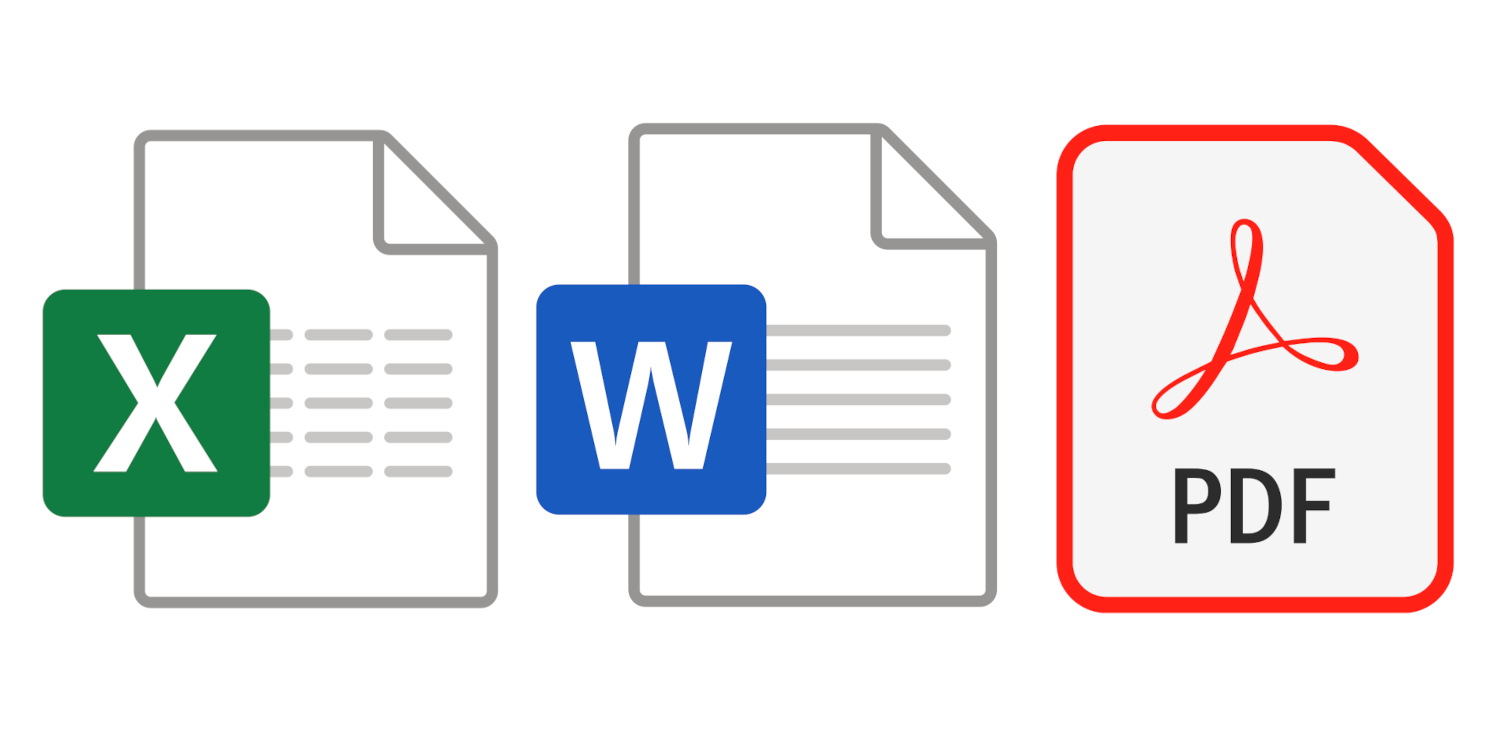
\includegraphics[alt={Logo docx, xlsx e pdf}, width=1\columnwidth]{img/format_logos.jpg}
	\caption{Logo formati documentali supportati}
	\label{fig:logos}
\end{figure}

Questo progetto ambizioso si propone inoltre di raggiungere i seguenti risultati:

\begin{itemize}
	\item \textbf{Semplificazione del processo:} ridurre la complessità nella creazione dei report, eliminando la necessità di gestire molteplici script isolati;
	\item \textbf{Incremento dell'efficienza:} accelerare il processo di generazione di report per nuovi casi specifici;
	\item \textbf{Standardizzazione:} implementare un approccio uniforme alla generazione dei report, facilitando la manutenzione e l'aggiornamento delle modalità di \textit{reporting};
	\item \textbf{Flessibilità:} creare una soluzione adattabile a diverse tipologie di dati e requisiti di \textit{reporting}, riducendo la necessità di sviluppare soluzioni \textit{ad hoc} per ogni nuovo caso d'uso;
	\item \textbf{Scalabilità:} progettare un sistema in grado di crescere e adattarsi alla diversificazione dei servizi offerti;
	\item \textbf{Base per future innovazioni:} fornire una piattaforma su cui costruire future espansioni o cambiamenti.
\end{itemize}

La realizzazione di questa libreria Python rappresenta quindi un passo verso l'ottimizzazione dei processi interni di RiskApp. Questo progetto non solo mira a risolvere le sfide immediate legate alla generazione dei report, ma si configura anche come un investimento per il futuro dell'azienda. 

In conclusione, questo progetto di stage si colloca all'intersezione tra l'ottimizzazione dei processi interni e l'innovazione tecnologica, riflettendo l'impegno che RiskApp pone nel miglioramento continuo dei propri servizi e rispondendo più efficacemente alle esigenze in continua evoluzione dei propri clienti.

\section{Motivi della scelta dell'attività di stage}
Il mio percorso verso lo stage in RiskApp è stato caratterizzato da una serie di circostanze favorevoli e scelte ponderate. A differenza di molti miei colleghi, non ho partecipato all'evento StageIT, ma sono entrato in contatto con l'azienda attraverso un canale differente.

RiskApp, ha attirato la mia attenzione per diversi motivi. In primo luogo, la dimensione ridotta dell'azienda e il suo ambiente dinamico promettevano un'esperienza di stage stimolante e ricca di opportunità di apprendimento. L'età media giovane del team e l'atmosfera energica che ne derivava rappresentavano per me un valore aggiunto significativo.

Ciò che ha reso l'approccio con RiskApp particolarmente interessante è stato il fatto che l'azienda stessa mi ha contattato, dimostrando interesse. Questo approccio proattivo da parte loro ha sicuramente influenzato positivamente la mia percezione dell'azienda e ha contribuito a farmi sentire valorizzato fin dall'inizio.

Durante i colloqui successivi, ho avuto modo di approfondire diversi aspetti cruciali:

\begin{itemize}
	\item \textbf{Il progetto di stage:} mi è stata presentata un'opportunità che si allineava perfettamente con i miei interessi e le mie competenze. Il progetto prevedeva lo sviluppo con tecnologie backend, un'area che mi appassiona particolarmente per la sua enfasi sulla logica e sulla risoluzione di problemi anche complessi;
	\item \textbf{Le tecnologie utilizzate:} la possibilità di lavorare con Django, un framework che avevo già intenzione di approfondire, ha rappresentato un forte incentivo. Questa opportunità mi avrebbe permesso di consolidare le mie competenze in un ambito di grande rilevanza nel mercato del lavoro attuale;
	\item \textbf{Il personale:} durante i colloqui, ho potuto apprezzare la cultura aziendale di RiskApp, il personale si è dimostrato da subito simpatico, disponibile e dotato di avanzate e affascinanti \textit{skill} professionali;
	\item \textbf{L'implementazione del progetto:} le discussioni preliminari sull'approccio tecnico al progetto mi hanno permesso di intravedere le sfide stimolanti che mi attendevano e di confermare la mia affinità con la metodologia di lavoro dell'azienda.
\end{itemize}

La decisione di accettare lo stage in RiskApp è stata ulteriormente rafforzata dalla buona reputazione di cui l'azienda gode nel settore. Inoltre, alcuni consigli positivi ricevuti da persone di fiducia hanno confermato la mia impressione iniziale sull'opportunità.

Ciò che ha definitivamente orientato la mia scelta è stata la natura del progetto proposto. L'opportunità di concentrarmi sullo sviluppo backend, evitando gli aspetti grafici che trovo meno stimolanti, si allineava perfettamente con le mie preferenze professionali. La prospettiva di lavorare su logiche anche complesse e strutture dati mi entusiasmava, promettendo un'esperienza di stage formativa e in linea con le mie aspirazioni future.

In conclusione, la combinazione di un ambiente giovane e dinamico, un progetto stimolante inerente allo sviluppo backend, e l'opportunità di approfondire tecnologie di mio interesse come Django, hanno reso RiskApp la scelta ideale per il mio stage. Questa esperienza si prospettava come un importante passo nel mio percorso di crescita professionale, promettendo una visione più concreta del mondo lavorativo nel settore IT.

\section{Vincoli}
	\subsection{Vincoli Tecnologici}
	
	L'attività di stage si svolge all'interno di un ecosistema tecnologico ben definito, caratterizzato da una serie di vincoli e specifiche che influenzano significativamente lo sviluppo del progetto. Questi vincoli, anche se lontani dall'essere limitazioni arbitrarie, riflettono le esigenze concrete dell'ambiente aziendale di RiskApp. Di seguito viene analizzato ciascun vincolo tecnologico, esplorandone le implicazioni e le ragioni sottostanti.
	
		\subsubsection{Python 3.7}
		Questa versione specifica del linguaggio di programmazione è stata scelta per garantire la massima compatibilità con l'ecosistema software di RiskApp e per allinearsi con le versioni di Django e altre dipendenze utilizzate nel progetto.
		
		L'adozione di Python 3.7 richiede un approccio strategico allo sviluppo:
		
		\begin{enumerate}
			\item \textbf{Gestione delle Dipendenze:} bisogna assicurarsi che tutte le librerie di terze parti utilizzate nel progetto siano compatibili con Python 3.7, usando precedenti versioni di esse quando richiesto;
			\item \textbf{Consapevolezza delle Limitazioni:} è necessaria una certa consapevolezza delle funzionalità disponibili in Python 3.7, evitando l'uso accidentale di sintassi o funzioni introdotte in versioni successive;
			\item \textbf{Futura evoluzione:} pur lavorando all'interno dei vincoli di Python 3.7, il codice deve essere quanto più compatibile con l'ultima versione disponibile (ad oggi la 3.12.4).
		\end{enumerate}
	
		\subsubsection{Django 2.2.4}
		Il framework Django, nella sua versione 2.2.4, è stato adottato come spina dorsale dei progetti RiskApp. Questa scelta specifica di versione è stata dettata principalmente da esigenze di intercompatibilità con gli strumenti e le infrastrutture preesistenti.
		
		Questa scelta richiede un approccio equilibrato allo sviluppo, sfruttando al massimo le potenzialità offerte da Django 2.2.4 mantenendo un occhio vigile sulle implicazioni di sicurezza dovute a possibili vulnerabilità note e performance.
		
		\subsubsection{XlsxWriter}
		Per la generazione di file Excel (formato .xlsx), si fa affidamento alla libreria XlsxWriter. Questa scelta è stata dettata dalla robustezza e dall'efficienza della libreria nel creare documenti Excel complessi e ricchi di funzionalità.
		
		La scelta di XlsxWriter è stata motivata dalla sua eccellente performance nella creazione di file da zero e dalla sua compatibilità con alcune specifiche funzioni di \gls{pandas} e l'architettura complessiva del progetto.
		
		\subsubsection{Python-docx}
		Questa libreria offre una \textit{Pythonic interface} per la manipolazione di documenti Word, consentendo la creazione di report strutturati e formattati secondo le esigenze aziendali.
		
		\subsubsection{Django REST Framework 3.10.3}
		Questo non rappresenta un vincolo in senso stretto, si è preferito operare in un \gls{playground} che implementasse \gls{drf} per garantire una maggior compatibilità della libreria con i sistemi di RiskApp.
		
		In modo analogo a Django, questa versione specifica è stata selezionata per garantire la massima compatibilità con l'ecosistema e le altre componenti software utilizzate da RiskApp.

	\subsection{Vincoli di Sviluppo e Test}
	Un vincolo cruciale del progetto è l'impossibilità di utilizzare dati proprietari dell'azienda durante lo sviluppo e i test. Questa restrizione, motivata da comprensibili esigenze di riservatezza e conformità normativa, porta inevitabilmente alla necessità di costruire un ambiente di sviluppo isolato detto \gls{playground}.
	
	Questo ambiente di test dedicato richiede:
	\begin{itemize}
		\item La creazione di un progetto Django indipendente, separato dai sistemi di RiskApp;
		\item la generazione di dati di test realistici ma anonimi, che mimassero la struttura e la complessità dei dati reali;
		\item l'implementazione di modelli di dati, viste e logiche di business simili a quelle usate nell'ambiente di produzione.
	\end{itemize}
	
	\subsection{Vincoli Temporali}


\section{Requisiti funzionali}
Un requisito fondamentale del progetto è l'assunzione che, come minimo, due argomenti dovessero essere forniti in input agli oggetti o funzioni responsabili della generazione dei report:
\begin{enumerate}
	\item \textbf{\textit{Django queryset}:} l'utilizzo di un \gls{queryset} come input primario garantisce una stretta integrazione con il modello dati dell'applicazione, permettendo query flessibili;
	\item \textbf{Configurazione:} definisce la struttura, il formato e i parametri specifici del report da generare. La configurazione è idealmente un \textit{blueprint} per il processo di generazione, determinando quali dati includere, come formattarli e come strutturare il documento finale.
\end{enumerate}

Questo approccio offre i seguenti vantaggi:
\begin{itemize}
	\item \textbf{Flessibilità:} permette di generare una varietà di report diversi utilizzando lo stesso set di dati, semplicemente dando in input diverse configurazioni;
	\item \textbf{Separazione delle preoccupazioni:} è presente una chiara distinzione tra i dati (\gls{queryset}) e la presentazione (configurazione), facilitando la manutenzione e l'evoluzione del sistema.
\end{itemize}

\newpage